\begin{figure}[!t]
	\hspace*{-4cm}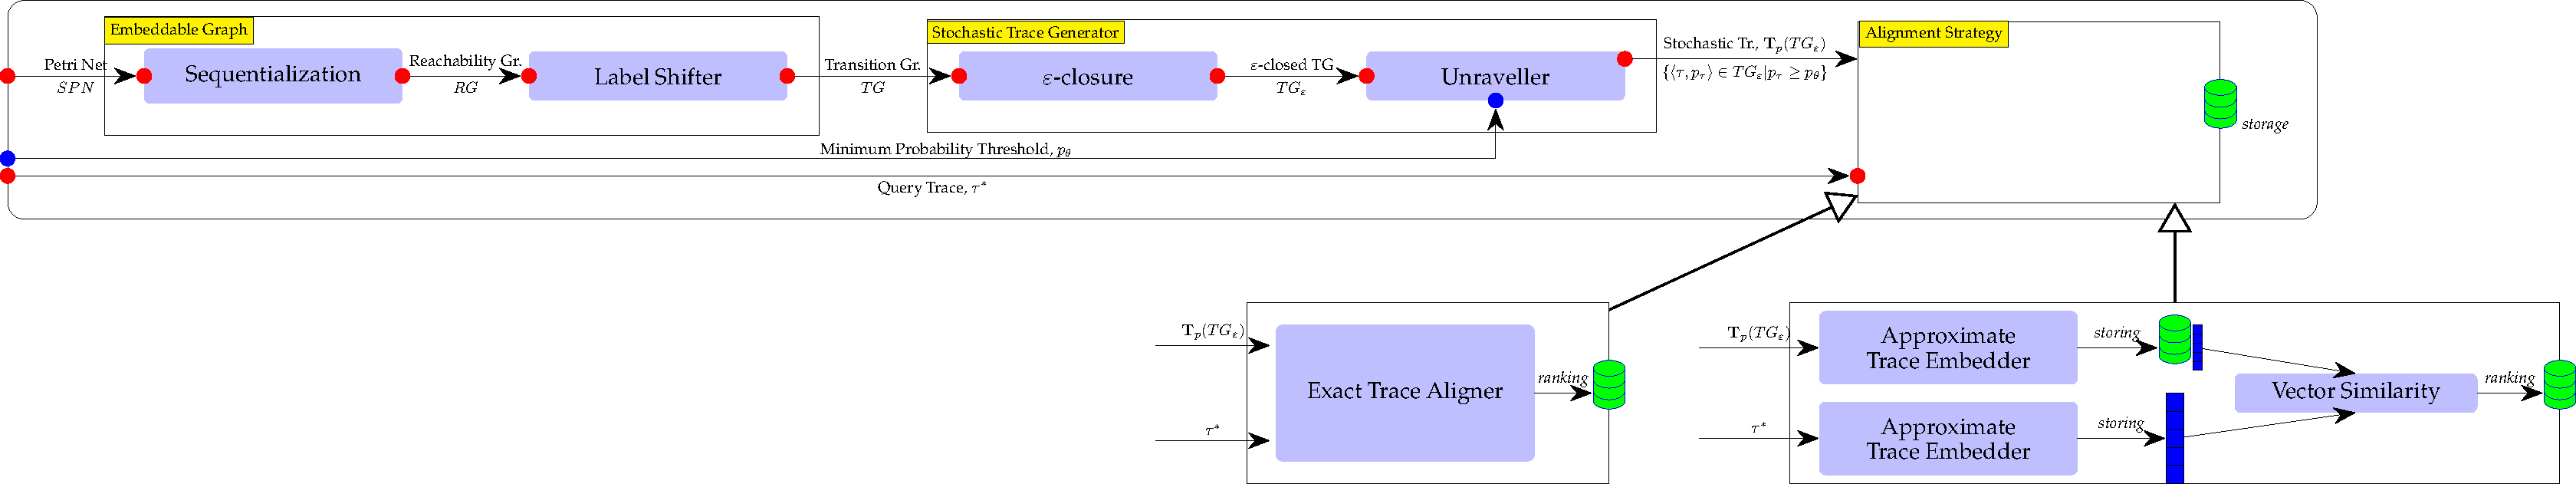
\includegraphics[width=1.7\textwidth]{images/pipeline}
	\caption{Proposed pipeline to assess the Probabilistic Trace Alignment}\label{fig:pipe}
\end{figure}


\section{Probabilistic Trace Alignment Pipeline}
This paper proposes the pipeline provided in Figure \ref{fig:pipe} by connecting several formalisations given in current literature via intermediate processing steps. The input of this pipeline is a query trace $\tau^*$ to be aligned, an Untimed Stochastic Workflow Net, and a minimum probability threshold $p_\theta$. The output of this pipeline is a set of model traces satisfying $p_\theta$ with an alignment ranking.

The pipeline is composed by the following phases: after representing the Untimed Stochastic Workflow Net as a graph of all the sequentially scheduled transitions (\S\ref{sec:seqZ}), we shift the labels from the edges towards the nodes while preserving the set of probabilistic traces (\S\ref{sec:LSift}) and minimize the graph representation by removing the $\varepsilon$-labelled nodes while preserving the traces' probability (\S\ref{sec:clos}). We extract the set of all the traces having $p_\theta$ as a minimum probability threshold (\S\ref{sec:unrav}) over which we're going to apply two different alignment strategies, the exact one (\S\ref{subsec:eta}) and the approximated one. 


Last, we are going to discuss how we can rank such traces in both the exact and the approximated scenario by reducing the alignment process to a k-nearest neighbour problem. While the exact trace alignment scenario requires to perform the alignment process each time a novel trace $\tau^*$ is introduced (\S\ref{subsec:exbkptap}), the approximated alignment allows to split the alignment into a preliminar loading phase and a query phase; in the former, each stochastic trace from the USWN is represented as a vector (\S\ref{subsec:ate}), and in the latter the to-be-aligned trace $\tau^*$ is first represented as a vector and then compared to all the other vectorial representations.  

\section{Sequentialization}\label{sec:seqZ}
In the sequentialization step, we transform a Untimed Stochastic Workflow Net with an initial marking $M$ into a Reachability Graph $(\mathcal{M},\mathcal{E})$ that is generated by the sequentialization process, where the potentially concurrent firing transitions are represented via a sequential scheduling. 

\begin{definition}[Reachability Graph]
	Given an initial marking $M$ for a Untimed Stochastic Workflow Net $USWN$,  the \textit{Reachability Graph} for $USWN$ is a graph $(\mathcal{M},\mathcal{E})$ where the nodes  $\mathcal{M}$ are composed of of all the reachable markings from $M$, $M$ included, and all the edges $\mathcal{E}$ are induced by the aforementioned relation $M\overset{t}{\to}M'$ among the reachability graph's nodes. To each of such edges $M\overset{t}{\to}M'$, we associate a transition probability $\mathbb{P}\left(M\overset{t}{\to}M'\right)=\frac{W(t)}{\sum_{t'\in E(M)}W(t')}$ \cite{spdwe}. 
\end{definition}

\begin{example}
Given a generic Untimed Workflow Net given in Figure \ref{fig:spn}, the Sequentialization process generates a Reachability Graph depicted in Figure \ref{fig:rg}: each node represents a marking $M$ as a vector, while the edges are labelled with the firing transitions. As we can see, the edges associated to this graph describes potentially concurrent firing transitions sequentially. While visiting the graph from $M$, the chaining of the edges' labels generates a trace generated from the Untimed Workflow Net, and the multiplication of the edges' weight provides the probability associated to the trace.
\end{example}



\section{Label Shifter}\label{sec:LSift}
Reachability Graphs generated via Sequentialization cannot be directly embedded using the embedding strategy proposed in current literature (\S\ref{ssec:ge}):  Reachability Graphs associated to Stochastic Workflow Nets are edge labelled, while Transition Graphs are Node Labelled. In order to represent the former as the latter, we need to shift the labels from the edges towards the nodes  while guaranteeing that such transformation preserves the set of the traces, as well as their associated probability. We provide such desired transformation in the following definition:

\begin{definition}[Label Shifter]\label{def:transf}
Given a Reachability Graph $(\mathcal{M},\mathcal{E})$ generated from an initial marking $M$, we can transform it into a Transition Graph $(s,t,L,R,1)$, where:
\begin{itemize}
	\item If there exist one single edge $M_1\overset{t}{\to}M_2\in\mathcal{E}$ where $M_1=M$, then $s=M\overset{t}{\to}M_2$; otherwise, we define a new node $\textbf{i}$ and we set it as the initial node for TG: $s=\textbf{i}$.
	\item If there exist one single edge $M_1\overset{t}{\to}M_2\in\mathcal{E}$ having no outgoing edges in the Reachability Graph, then $t=M_1\overset{t}{\to}M_2$; otherwise, we define a new node $\textbf{f}$ and we set it as the accepting node for TG:  $t=\textbf{f}$.
	\item $[L]_{\lambda(t),\;M\overset{t}{\to} M'}=1$ for each $M\overset{t}{\to} M'\in\mathcal{E}$; if $\textbf{i}$ is defined then $[L]_{\varepsilon\textbf{i}}=1$; if $\textbf{f}$ is defined, then $[L]_{\varepsilon\textbf{f}}=1$; $[L]_{ij}=0$ otherwise.
	\item $[R]_{M\overset{t}{\to} M',\;M'\overset{t'}{\to} M''}=\frac{W(t')}{\sum_{\textbf{t}\in E(M')}W(\textbf{t})}$ for each $M\overset{t}{\to} M',M'\overset{t'}{\to} M''\in\mathcal{E}$; if $\textbf{i}$ is defined, then $[R]_{\textbf{i},\;M\overset{t}{\to}M'}=\frac{W(t)}{\sum_{\textbf{t}\in E(M)}W(\textbf{t})}$; if $\textbf{f}$ is defined, then $[R]_{M\overset{t}{\to}M',\;\textbf{i}}=1$ for each $M'$ having no outgoing edges in the Reachability Graph; $[R]_{ij}=0$ otherwise.
\end{itemize}
\end{definition}

We can also show that the Transition Graph obtained in Definition \ref{def:transf} preserves the same set of probabilistic traces associated by the Reachability Graph, but the proof of such claim  is omitted due to the lack of space.

\begin{example}
Figure \ref{fig:lmc} provides the output of such transformation if Figure \ref{fig:rg} is used as an input. All the nodes are labelled using the firing transitions' labels (in green), while the edges preserve the probabilistic information from the Reachability Graph (in red). Intuitively, when a new initial node \textit{\textbf{i}} is inserted, we preserve all the initial probabilistic choices that a transition is fired from an initial marking $M$, while all the intermediate edges inherit the probabilisitc choice of the firing transition from the subsequent choices. When a new final node \textit{\textbf{f}} is added, such edges always have probability $1$, and therefore we do not interfere with the initial traces' probability.
\end{example}

\section{$\varepsilon$-closure}\label{sec:clos}
The $\varepsilon$-closure process has two main purposes: first, it reduces the size of the Transition Graph generated in the previous step by removing all the $\varepsilon$-labelled nodes \texttt{\color{blue}w} and preserving the connection between  the nodes \texttt{\color{blue}u} from its ingoing edges   $\texttt{\color{blue}u}\xrightarrow{\color{red}p_i}\texttt{\color{blue}w}$ with the nodes \texttt{\color{blue}v} from its ingoing edges   $\texttt{\color{blue}w}\xrightarrow{\color{red}p_j}\texttt{\color{blue}v}$ by establishing new edges $\texttt{\color{blue}u}\xrightarrow{\color{red}p_ip_j}\texttt{\color{blue}v}$. $\varepsilon$-labelled initial (or accepting) nodes are removed if and only if they have only one outgoing (ingoing) edge with probability $1$.

\begin{example}
	The $\varepsilon$-closure remotes the non-initial and non-accepting nodes within such automaton, while preserving the probabilistic trace equivalence of the two automata: node \texttt{\color{blue}10} is then removed alongside its associated edges, and new edges $\texttt{\color{blue}3}\xrightarrow{\color{red}p_4}\texttt{\color{blue}4}$ and $\texttt{\color{blue}3}\xrightarrow{\color{red}p_5}\texttt{\color{blue}5}$ are introduced. The resulting TG $P$ is represented with the same graphical depiction Figure \ref{fig:closed}.
\end{example}

Consequently, it is always possible to minimize a TG  (e.g., Figure \ref{fig:orig}) via $\varepsilon$-closure, so that the only nodes that are labelled as $\varepsilon$ are the source and the target nodes (Figure \ref{fig:closed}) and the set of weighted traces is preserved. From now on, we always that all the TGs are minimized via $\varepsilon$-closure. 

\section{Unraveller}\label{sec:unrav}
Being that both the graph isomorphism problem is NP-Complete and the TGs are fully characterized by the set of the probabilistic traces that they generate,  we can say that two TGs are (probabilistic-trace) equivalent if and only if they share the same set of weighted traces. In particular, we denote as $\mathcal{W}_p(P)$ the set of all the weighted traces in $P$ having at least probability $p$. Under these assumptions, the probabilistic trace equivalence is deterministic.

\begin{example}
	The TG in Figure \ref{fig:orig} has the following set $\mathcal{W}_0(P^*)$ of weighted traces:
$$\set{\braket{\underbrace{\color{green}a\dots a}_{n},{\color{red}p_1p_3^np_6}}|n\in \mathbb{N}_{>0}}\cup \set{\braket{{\color{green}c}\underbrace{\color{green}a\dots a}_{n},{\color{red}p_2p_4p_3^np_6}}|n\in \mathbb{N}_{>0}}\cup\{\braket{{\color{green}cb},{\color{red}p_2p_5}}\}$$
We can easily see that, after the $\varepsilon$-closure process, $\mathcal{W}_0(P^*)=\mathcal{W}_0(P)$, so the two TGs are (probabilistic-trace) equivalent.
\end{example}

\section{Alignment Strategy}

\subsection{Exact Trace Aligner}\label{subsec:eta}
\ADD{A possible way to carry out probabilistic trace alignment is to reuse existing trace aligners such as \cite{LeoniM17}, where the alignment outcome is usually  expressed as a distance function $d(\tau,\tau^*)$. Therefore, we can exploit decision theory at first \cite{dectheor} and express the statistical decision of aligning a weighted trace $\braket{\tau,w_\tau}\in\mathcal{W}_{p_\theta}(P)$ with $\tau^*$ as the weighted cost of performing a (bad) alignment $w_\tau d(\tau,\tau^*)$. If we want to represent the same intuition of such weighted cost as a kernel function (\S\ref{subsec:katk}) so to compare such strategy to our proposed approximate trace embedder, we need to transform it as a function returning $1$  when $\tau$ is the desired trace with probability $w_\tau=1$ and $\tau=\tau^*$. In order to do so, we might prefer to express $d$ as}
\xout{We can express our probabilistic trace alignment as finding the trace that maximizes both the trace's probability and its similarity with the query trace $\tau^*$. Still, the trace alignments problems are usually expressed via trace alignments cost functions, and not via trace similarities \cite{LeoniM17}. Given a generic trace cost function $d(\tau,\tau')$, it is always possible to convert it into} a normalized similarity score $s_d(\tau,\tau'):=1/(d(\tau,\tau')/c+1)$ where $c\in\mathbb{N}_{\neq 0}$ is a constant, so that the maximum similarity of $1$ is reached when the distance is $0$ and the similarity decreases while the distance increases \cite{BergamiBM20}. \xout{As a consequence, the exact trace aligner will find the weighted trace $\braket{\tau,\mathbb{P}(\tau)}$ in $\mathcal{W}_{p_\theta}(P)$ maximising $s_d(\tau,\tau^*)$, and use $s_d$ as a ranking function.} \ADD{Given that usually $w_{\tau^*}=1$, we can express the golden kernel function $k_\star$ as $k_\star(\tau,\tau^*)=w_\tau w_{\tau^*} s_d(\tau,\tau^*)$: we are going to use this function to both } \xout{Section \ref{subsec:exbkptap} is going to discuss how such problem might be} reduce\xout{d} \ADD{it} to the k-nearest neighbour problem\ADD{ (\S\ref{subsec:exbkptap}), and compare this ranking to the one induced by the approximated vectorial embedding (\S\ref{sec:exp}) proposed in the incoming subsection.}

\subsection{Approximate Trace Embedder}\label{subsec:ate}
\ADD{We want to define an embedding $\mathcal{P}$ for a dot-product-based kernel $k_{\mathcal{P}}$ so that it almost performs ideally (\S\ref{subsec:katk} and \cite{Gartner03}). Given that the embedding of a (weighted) trace $\braket{\tau,w_\tau}\in\mathcal{W}_{p_\theta}(P)$ requires an intermediate $TG$ representation, we can map each of these traces to the subgraph of $P$ generating $\braket{\tau,w_\tau}$ with at most $|\tau|$ steps:}
	\begin{definition}[Trace Embedding for TGs]
		Given a minimum probability\\ threshold $p_\theta$ \xout{, a maximum path length $n$,} and a TG $P=(s,t,L,R,w)$, we generate the set of the trace embeddings for $P$ as follows: for each weighted trace $\braket{\tau,w_\tau}\in\mathcal{W}_{p_\theta}(P)$ generated from a path $\pi_\tau=s\to n_2\rightsquigarrow n_m\to t$ over $R$, we generate a TG $P_\tau=(s',t',L_\tau,R_\tau,w_\tau)$, where \begin{alphalist}
			\item $s'=s$ if $\textit{label}(s)\neq \varepsilon$ and $t'=n_2$ otherwise,
			\item $t'=t$ if $\textit{label}(t)\neq \varepsilon$ and $t'=n_m$ otherwise,
			\item $L_\tau$ (and $R_\tau$) is the submatrix of $L$ (and $R$) over the non-$\varepsilon$ labelled notes in $\pi_\tau$ and the labels from $\tau$,
			\item $w'$ is initialised by $w$ and then multiplied by $[R]_{s,n_2}$ (and also $[R]_{n_m,t}$) if $\textit{label}(s)=\varepsilon$ (and  $\textit{label}(t)=\varepsilon$).
		\end{alphalist}
			\begin{enumerate}
			\item \xout{each $P_\tau$ is then represented as $\phi_{\mathcal{P}}(P_\tau)$ and added to the set $\mathbf{T}_p^n(P)$.}
		\end{enumerate}
	\end{definition}

\begin{table}[!t]
	\caption{Generating the sub-TGs $P_\tau\in \mathbf{T}_0^4(P)$ from the TG $P$ via the set of weighted traces $\mathcal{W}_0^4(P)$. $l$ and $w$ respectively represent the desired parameter for $\phi_{\mathcal{P}}(P_\tau)$ and the weight associated to $P_\tau$.}\label{tab:proj}
	\centering
	\resizebox{.45\textwidth}{!}{\begin{tabular}{>{\centering\arraybackslash} m{1cm}| >{\centering\arraybackslash} m{4cm} >{\centering\arraybackslash} m{1cm} >{\centering\arraybackslash} m{1cm} }
			\toprule
			$\tau$&$P_\tau$&$l$&$w$\\
			\midrule
			a & 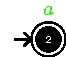
\includegraphics{images/trace_a} & $1$ & $\color{red}p_1p_6$\\
			cb & 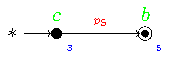
\includegraphics{images/trace_cb} & $2$ & $\color{red}p_2$\\
			aaa & 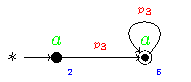
\includegraphics{images/trace_a_loop} & $3$ & $\color{red}p_1p_6$\\
			caa & 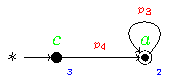
\includegraphics{images/trace_ca_loop} & $3$ & $\color{red}p_2p_6$\\
			\bottomrule
	\end{tabular}} 	\resizebox{.45\textwidth}{!}{\begin{tabular}{>{\centering\arraybackslash} m{1cm}| >{\centering\arraybackslash} m{4cm} >{\centering\arraybackslash} m{1cm} >{\centering\arraybackslash} m{1cm} }
	\toprule
	$\tau$&$P_\tau$&$l$&$w$\\
	\midrule
	aa & 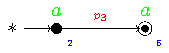
\includegraphics{images/trace_aa} & $2$ & $\color{red}p_1p_6$\\
	ca & 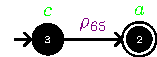
\includegraphics{images/trace_ca} & $2$ & $\color{red}p_2p_6$\\
	\begin{tabular}{l}aaaa\end{tabular} & 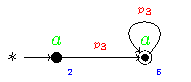
\includegraphics{images/trace_a_loop} & $4$ & $\color{red}p_1p_6$\\
	caaa & 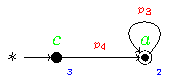
\includegraphics{images/trace_ca_loop} & $4$ & $\color{red}p_2p_6$\\
	\bottomrule
\end{tabular}}
\end{table} 
\begin{example}\label{ex:neue}
Given the TG $P$ in Figure \ref{fig:closed}, we assign the following probability values to the edges: $p_1=0.8$, $p_2=0.2$, $p_3=p_6=0.5$, $p_4=0.7$, and $p_5=0.3$. If we limit our analysis to all the traces of maximum length $4$, we generate the following probabilistic traces set:
$$\begin{aligned}
\{&\braket{a,0.4},\braket{aa,0.2},\braket{aaa,0.1},\braket{ca,0.07},\\
&\braket{cb,0.06},\braket{aaaa,0.05},\braket{caa,0.035},\braket{caaa,0.0175}\}\\
\end{aligned}$$
\medskip

Table \ref{tab:proj} represents the TGs $P_\tau\in\mathbf{T}_p^n(P)$ with weight $w$ generated for each weighted path $\braket{\tau,w_\tau}\in \mathcal{W}_0^4(P)$ of length $l=|\tau|$ from the TG $P$ in Figure \ref{fig:closed}. The associated weight $w$ derives from the source's outgoing edges (and target's ingoing edges) when such node is labelled as $\varepsilon$: given that the selection of a trace $\tau$ implies performing a set of specific probabilistic choices, we can remove all the edges starting (and arriving) at nodes that are $\varepsilon$-labelled and move their score as the weight of the TG.
\end{example}
	
	\ADD{We can now focus on the embedding $\phi_{\mathcal{P}}$ for each TG associated to our selected weighted traces. The main goal is use $k_{\mathcal{P}}$ for ranking all the traces generated by the Unravelling step. Walking on such footsteps, we now want to extend such previous work by both including the traces' associated probability and by making the ranking induced by $k_{\mathcal{P}}$ the inverse of the sum of the following distances: the transitions correlations $\epsilon$ and the transitions' label frequency $\nu$. }
\xout{Given that we previously observed that a TGs $P$ can be fully characterised (read, similarity) by their associated set of traces $\mathcal{W}_p^n(P)$  and that the trace embedding can be described as an embedding over a TG, we can characterise a TG embedding as a transition matrix embedding. In addition to that, when two Workflow Nets share similar node labellings but no ${\color{green}\alpha}\rightsquigarrow{\color{green}\beta}$ paths for any ${\color{green}\alpha}$ and ${\color{green}\beta}$, we should combine the former embedding with an embedding characterising the frequency on how the nodes' labels appear in the generated traces.} \ADD{We would also require that the desire properties of $\phi_{\mathcal{P}}$ is independent from the characterization of $\epsilon$ and $\nu$, which would only provide different embedding strategies. } We can now provide the following definition:


%\begin{table}[!t]
%	\centering
%	\caption{Embedding representation for the TG $P$ in Figure \ref{fig:closed} and the trace $\tau^*=\textup{caba}$ after representing it as in Figure \ref{fig:taustar}. Please note that we restrict $\Sigma_\varepsilon^2$ to the one from $P$.}\label{tab:emb1}
%		\begin{tabular}{l|l|l|l|l|l|l|}
%	\toprule
%	& a    & b                                                   & c    & aa   & ca   & cb   \\
%	\midrule
%	$\phi_{\mathcal{P}}(P)$ & $9.94\cdot10^{-25}$ & $1.18\cdot 10^{-26}$ & $1.04\cdot10^{-25}$ & $4.45\cdot 10^{-25}$ & $6.22\cdot10^{-25}$ & $8.29\cdot10^{-26}$\\
%	$\phi_{\mathcal{P}}(T)$ & $8.16\cdot10^{-17}$ & $4.08\cdot 10^{-17}$ & $4.08\cdot10^{-17}$ & $4.37\cdot 10^{-17}$ & $1.03\cdot10^{-16}$ & $4.37\cdot10^{-17}$\\
%	\bottomrule
%\end{tabular}
%\end{table}
\begin{definition}[TG Embedding]\label{def:ppne}
Given a finite set of non-empty labels $\Sigma_\varepsilon =\Sigma\backslash\{\varepsilon\}$, $\Sigma_\varepsilon^2$ denotes all the possible pair of labels associated to paths ${\color{green}\alpha}\rightsquigarrow{\color{green}\beta}$ and $\Sigma_\varepsilon$ denotes the set of all the possible non-$\varepsilon$ node labels. Therefore, it is always possible to enumerate $\Sigma_\varepsilon^2\cup\Sigma_\varepsilon$ via an enumeration by a bijection $\iota\colon \Sigma_\varepsilon^2\cup\Sigma_\varepsilon\to  N$, where $N\subset \mathbb{N}_{\neq 0}$ and $\max N=|N|$.
	
Given a TG $P=(s,t,L,R,w)$ resulting from a $\varepsilon$-closure and a tuning parameter $t_f\in[0,1]\subseteq\mathbb{R}$, the associated embedding is defined as follows:
$$\phi_{\mathcal{P}}(P)_i=\begin{cases}
	\frac{\epsilon(P)_{\color{green}\alpha\beta}}{\|\epsilon\|_2}wt_f^{|R>0|} & i={\color{green}\alpha\beta}\\
	\frac{\nu(P)_{\color{green}\alpha}}{\|\nu\|_2}t_f^{|R>0|} & i={\color{green}\alpha}\\
\end{cases}$$
where $\epsilon$ and $\nu$ respectively represent the non-negatively defined embedding associated to the TG's transition matrix and nodes. 
\end{definition}

Albeit the definition of $\epsilon$ and $\nu$ might vary, we choose a specific definition for them. 
We can define the transition matrix embedding as follows:
\begin{equation}\label{eq:epsilon}
\epsilon(P)_{\color{green}\alpha\beta}=\sum_{i=1}^l{\lambda^i}\frac{[LR^iL^t]_{\color{green}\alpha\beta}}{\sum_{\color{green}\alpha'\beta'}R^i_{\color{green}\alpha'\beta'}}
%
\end{equation}
\begin{equation}\label{eq:nu}
\nu(P)_{\color{green}\alpha}=\frac{1}{N}\sum_{\braket{\tau,w}\in\mathcal{W}_p^l(P)}\frac{|\Set{\tau_i\in\tau|\tau_i\neq\varepsilon\wedge \tau_i={\color{green}\alpha}}|}{|\tau|}
\end{equation}
where $l$ is the maximum path length that we want to consider as valid, and $N$ is a normalization factor such that $\sum_{{\color{green}\alpha}\in\Sigma_\varepsilon}\nu(R,L)_{\color{green}\alpha}=1$. In Example \ref{ex:cmpexample} we will see that the given definition of $\epsilon$ provides a better approximation than the edge embedding given in current literature (\S\ref{subsec:katk}), i.e. $\tilde{\epsilon}(P)_{\color{green}\alpha\beta}=\sum_{i=1}^l\lambda^i[\Lambda^i]_{\color{green}\alpha\beta}$.


%When the transition matrix is ergodic \cite{StocasticCC},  the transition matrix embedding converges to $\epsilon(R)_{\color{green}\alpha\beta}=[(\mathbf{I}-\lambda\Lambda)^{-1}]_{\color{green}\alpha\beta}$ \cite{GartnerFW03} for $n\to+\infty$.

\begin{table}[!t]
	\centering
	\caption{Embedding for all the traces of maximum length $4$ generated from $P$.}\label{tab:emb2}
	\begin{tabular}{l|l|l|l|l|l|l|}
		\toprule
		& a    & b                                                   & c    & aa   & ca   & cb   \\
		\midrule
		
		
		$\phi_{\mathcal{P}}(P_\textup{aaaa})$ & $1.00\cdot 10^{-24}$ & $0.00\cdot 10^{0}$ & $0.00\cdot 10^{0}$& $6.44\cdot 10^{-26}$& $0.00\cdot 10^{0}$& $0.00\cdot 10^{0}$\\
		$\phi_{\mathcal{P}}(P_\textup{aaa})$ & $1.00\cdot 10^{-24}$ & $0.00\cdot 10^{0}$ & $0.00\cdot 10^{0}$& $1.29\cdot 10^{-25}$& $0.00\cdot 10^{0}$& $0.00\cdot 10^{0}$\\
		$\phi_{\mathcal{P}}(P_\textup{aa})$ & $1.00\cdot 10^{-24}$ & $0.00\cdot 10^{0}$ & $0.00\cdot 10^{0}$& $2.57\cdot 10^{-25}$& $0.00\cdot 10^{0}$& $0.00\cdot 10^{0}$\\
		$\phi_{\mathcal{P}}(P_\textup{a})$ & $1.00\cdot 10^{-4}$ & $0.00\cdot 10^{0}$ & $0.00\cdot 10^{0}$& $0.00\cdot 10^{0}$& $0.00\cdot 10^{0}$& $0.00\cdot 10^{0}$\\
		$\phi_{\mathcal{P}}(P_\textup{caa})$ & $7.07\cdot 10^{-25}$ & $0.00\cdot 10^{0}$ & $7.07\cdot 10^{-25}$& $1.46\cdot 10^{-25}$& $2.05\cdot 10^{-25}$& $0.00\cdot 10^{0}$\\
		$\phi_{\mathcal{P}}(P_\textup{ca})$ & $7.07\cdot 10^{-25}$ & $0.00\cdot 10^{0}$ & $7.07\cdot 10^{-25}$& $0.00\cdot 10^{0}$& $1.00\cdot 10^{-8}$& $0.00\cdot 10^{0}$\\
		$\phi_{\mathcal{P}}(P_\textup{cb})$ &  $0.00\cdot 10^{0}$ & $7.07\cdot 10^{-25}$ & $7.07\cdot 10^{-25}$& $0.00\cdot 10^{0}$&  $0.00\cdot 10^{0}$ & $4.29\cdot 10^{-9}$\\
		$\phi_{\mathcal{P}}(P_\textup{caaa})$  & $7.07\cdot 10^{-25}$ &  $0.00\cdot 10^{0}$ & $7.07\cdot 10^{-25}$& $1.03\cdot 10^{-25}$&  $7.20\cdot 10^{-26}$ & $0.00\cdot 10^{0}$\\
		\bottomrule
	\end{tabular}
\end{table}
\begin{example}\label{ex:withpaths} Given $\Sigma_\varepsilon=\Set{a,b,c}$ and $V=\set{1,2,3,5,6}$, we have that all the embedding space should be at least of size $6$, as $\{a,b,c,aa,ca,cb\}\subseteq \Sigma_\varepsilon^2\cup\Sigma_\varepsilon$ is the whole set of features describing both the transition matrix and the nodes. We chose $t_f=0.0001$, $\lambda=0.7$ for our embedding strategy. 

\xout{The embedding associated to $P$ is described in Table \ref{tab:emb1} as $\phi_{\mathcal{P}}(P)$: it shows that doing ${\color{green}a}\rightsquigarrow{\color{green}a}$ is more probable than doing  ${\color{green}c}\rightsquigarrow{\color{green}a}$. Also, given that both the probability of performing ${\color{green}c}\overset{1}{\rightsquigarrow}{\color{green}b}$ is relatively low and trace $\color{green}cb$ is relatively infrequent, ${\color{green}c}{\rightsquigarrow}{\color{green}b}$ is less probable than any other subtrace. If we now consider the single nodes, $\color{green}c$ shares a subset of traces with $\color{green}a$ where $\color{green}a$ is more frequent than $\color{green}c$, and therefore the score of the former is higher than the one of the latter. Also, the score associated to the single node $\color{green}b$ is lower than the one for the single node $\color{green}c$ because $\color{green}b$ is less frequent and appears in less probable traces than $\color{green}c$: in particular, $\color{green}c$ appears in \textit{ca}, which is more probable than \textit{cb}.}

\ADD{After representing trace $\tau^*=\textup{caba}$ to be aligned as a graph (see Example \ref{ex:tracembed}), we can represent its}
\xout{Similar considerations can be also drawn from the} embedding $\phi_{\mathcal{P}}(T)$ \xout{associated to the trace $\tau^*=\textup{caba}$ (also in Table --):} \ADD{as follows:}
		\begin{tabular}{l|l|l|l|l|l|l|}
	\toprule
	& a    & b                                                   & c    & aa   & ca   & cb   \\
	\midrule
%	$\phi_{\mathcal{P}}(P)$ & $9.94\cdot10^{-25}$ & $1.18\cdot 10^{-26}$ & $1.04\cdot10^{-25}$ & $4.45\cdot 10^{-25}$ & $6.22\cdot10^{-25}$ & $8.29\cdot10^{-26}$\\
	$\phi_{\mathcal{P}}(T)$ & $8.16\cdot10^{-17}$ & $4.08\cdot 10^{-17}$ & $4.08\cdot10^{-17}$ & $4.37\cdot 10^{-17}$ & $1.03\cdot10^{-16}$ & $4.37\cdot10^{-17}$\\
	\bottomrule
\end{tabular}
${\color{green}a}$ is clearly the most frequent label ${\color{green}b}$ and ${\color{green}c}$ are equiprobable, as well as the path ${\color{green}c}\rightsquigarrow {\color{green}a}$ appears twice in the trace's set and then, it is more frequent than the other subtraces. \ADD{Similar considerations can be followed for possibly embedding the whole transition graph $P$.}

\xout{Last, we can observe that the representation of $\phi_{\mathcal{P}}$ only depends on the $\Sigma_\varepsilon$ of choice and on the TG that we want to represent. As a consequence, this representation is entirely independent of the alignment that we might be interested in calculating in a subsequent step.}

 Table \ref{tab:emb2} represents the embeddings $\phi_{\mathcal{P}}(P_\tau)$ generated from the sub-TGs generated in Example \ref{ex:neue}, where the $l=|\tau|$ for each trace $\tau$ associated to the sub-TG. \xout{As we can see,} This representation is completely independent from the representation associated with a trace to be aligned. Therefore it doesn't have to be recomputed at each alignment with a different $\tau^*$.
\end{example}

\xout{After defining the embedding, we can show that this embedding establishes some desired features that are independent of the definition of $\epsilon$ and $\nu$, and that $\epsilon$ and $\nu$ only depend on the characterization of both the labelling $L$ and the transition matrix $R$. We provide a rewriting proposition that is going to be used in the incoming subsection to provide the aforementioned characterizing properties.} \ADD{We can prove some of our desired features after rewriting the former definition via the distance between the vectorial representations of $\epsilon$ and $\nu$:}


\begin{proposition}\label{lem:rewritinglemma}
Given two TGs $P=(s,t,L,R,w)$ and $P'=(s',t',L',R',w')$, the TG Kernel is defined as follows:
$$\begin{aligned}
k_{\phi_{\mathcal{P}}}(P,P')=&ww't_f^{|R>0|+|R'>0|}\left(1-\frac{\norm{\hat{\epsilon}-\hat{\epsilon}'}{2}^2}{2}\right)+\\
	&+t_f^{|R>0|+|R'>0|}\left(1-\frac{\norm{\hat{\nu}-\hat{\nu}'}{2}^2}{2}\right)\\
\end{aligned}$$
\end{proposition}
\begin{proof}
$$\begin{aligned}
\Rcancel{k_{\phi_{\mathcal{P}}}(P,P')}&\Rcancel{=\Braket{\phi_{\mathcal{P}}(P),\phi_{\mathcal{P}}(P')}}\\
	&\Rcancel{=\sum_{\alpha\beta\in \Sigma_\varepsilon^2}\frac{\epsilon_{\color{green}\alpha\beta}}{\|\epsilon\|_2}\frac{{\epsilon'}_{\color{green}\alpha\beta}}{\|\epsilon'\|_2}ww't_f^{|R>0|+|R'>0|}\quad+\quad \sum_{\alpha\in \Sigma_\varepsilon}\frac{\nu_{\color{green}\alpha}}{\|\nu\|_2}\frac{{\nu'}_{\color{green}\alpha}}{\|\nu'\|_2}t_f^{|R>0|+|R'>0|}}\\
	&\Rcancel{=ww'\tau^{|Rb>0|+|R'>0|}\sum_{\alpha\beta\in \Sigma_\varepsilon^2}\frac{\epsilon_{\color{green}\alpha\beta}}{\|\epsilon\|_2}\frac{{\epsilon'}_{\color{green}\alpha\beta}}{\|\epsilon'\|_2}\quad+\quad t_f^{|R>0|+|R'>0|}\sum_{\alpha\in \Sigma_\varepsilon}\frac{\nu_{\color{green}\alpha}}{\|\nu\|_2}\frac{{\nu'}_{\color{green}\alpha}}{\|\nu'\|_2}}\\
	&\Rcancel{=ww't_f^{|R>0|+|R'>0|}\Braket{\hat{\epsilon}, \hat{\epsilon}'}+ t_f^{|R>0|+|R'>0|}\Braket{\hat{\nu}, \hat{\nu}'}}\\
	&\Rcancel{=ww't_f^{|R>0|+|R'>0|}\left(1-\frac{\norm{\hat{\epsilon}- \hat{\epsilon}'}{2}^2}{2}\right)+ t_f^{|R>0|+|R'>0|}\left(1-\frac{\norm{\hat{\nu}- \hat{\nu}'}{2}^2}{2}\right)}\\
\end{aligned}$$
\end{proof}

\xout{Given that we can now follow Definition \ref{def:ppne} for representing a trace $\tau$ as a proper embedding after transforming it as a TG $T$ (\S\ref{subsec:katk}), we can find the TG $P$ providing the best approximate match with  a trace $\tau$ as follows:}
\[\Rcancel{\underset{{P}}{\max\arg}\;k_{\phi_{\mathcal{P}}}(P,T)}\]
\xout{Still, this TG matching strategy does not allow to find the trace maximizing such score.} %To assess such problem, the next section is going to determine both an exact (\S\ref{subsec:exbkptap}) and an approximated strategy (\S\ref{subsec:akptap}) for probabilistically matching one single trace from the TG.

\xout{Given the characterization of a TG as in \S\ref{subsec:ppn} and the embedding strategy proposed in Definition \ref{def:ppne}, We can \ADD{now} generate an embedding for each possible weighted trace $\braket{\tau,w_\tau}\in\mathcal{W}_p^n(P)$ for a given TG $P$ as described in the following definition:}





\begin{table}[!t]
	\caption{Comparison between the ranking induced by the kernel function and the expected ranking $k_\star$: the rows are sorted by $k_{\phi_{\mathcal{P}}}$ descending order. The largest similar ranking subsequence is marked in blue.}\label{tab:rank3}
	\centering
	%	\begin{tabular}{l|c|ll}
	%		\toprule
	%		$\tau$ & $k_{\phi_{\mathcal{P}}}(\tau,\tau^*)$ & \textit{kernel ranking} & expected ranking\\
	%		\midrule
	%		a & $8.16\cdot 10^{-21}$ & \textbf{1} & \textbf{\color{blue}1}\\
	%		ca & $1.89\cdot 10^{-24}$ & \textbf{2} & \textbf{\color{blue}4}\\
	%		cb & $7.64\cdot 10^{-25}$ & \textbf{3} & \textbf{\color{blue}5}\\
	%		caa & $1.14\cdot 10^{-40}$ & \textbf{4} & \textbf{\color{blue}7}\\
	%		caaa & $9.84\cdot 10^{-41}$ & \textbf{5} & \textbf{\color{blue}8}\\
	%		aa & $9.28\cdot 10^{-41}$ & \textbf{6} & \textbf{\color{red}2}\\
	%		aaa & $8.72\cdot 10^{-41}$ & \textbf{7} & \textbf{\color{red}3}\\
	%		aaaa & $8.44\cdot 10^{-41}$ & \textbf{8} & \textbf{\color{red}6}\\
	%		
	%		\bottomrule
	%	\end{tabular}
	
	\begin{tabular}{lc|ll|cc|l}
		\toprule
		
		\multirow{2}{*}{$\tau$} &
		\multirow{2}{*}{$d(\tau,\tau^*)$} &
		\multicolumn{2}{c|}{$\mu_{\tau^*}$} &
		\multirow{2}{*}{$\approx s_d(\tau,\tau^*)\cdot w_\tau$} &
		\multirow{2}{*}{$k_{\phi_{\mathcal{P}}}(P_\tau,T)$}&
		\multirow{2}{*}{$k_\star(\tau,\tau^*)$}\\
		
		\cline{3-4} &&  $\langle w_\tau$ &  $,\,s_d(\tau,\tau^*)\rangle $ && \\
		
		\midrule
		{a}  & $3$ & $0.4$ & $\;\; 0.6250$  & $0.2500$ & $8.16\cdot 10^{-21}$ & \textbf{\color{blue}1}\\
		{ca}  & $2$ & $0.07$ & $\;\; 0.7142$ & $0.0500$ & $1.89\cdot 10^{-24}$ & \textbf{\color{blue}4}\\
		{cb}  & $2$ & $0.06$ & $\;\; 0.7142$ & $0.0428$ & $7.64\cdot 10^{-25}$ & \textbf{\color{blue}5}\\
		{caa}  & $1$ & $0.035$ & $\;\; 0.8333$ & $0.0292$ & $1.14\cdot 10^{-40}$ & \textbf{\color{blue}7}\\
		{caaa}  & $1$  & $0.0175$ & $\;\; 0.8333$ & $0.0145$ & $9.84\cdot 10^{-41}$ & \textbf{\color{blue}8}\\
		{aa}  & $2$ & $0.2$ & $\;\; 0.7142$ & $0.1428$ & $9.28\cdot 10^{-41}$ & \textbf{\color{red}2}\\
		{aaa}  & $2$ & $0.1$ & $\;\; 0.7142$ & $0.0714$ & $8.72\cdot 10^{-41}$ & \textbf{\color{red}3}\\
		{aaaa}  & $3$ & $0.05$ & $\;\; 0.0357$ & $0.0357$ & $8.44\cdot 10^{-41}$ & \textbf{\color{red}6}\\
		\bottomrule
	\end{tabular}
\end{table}


At this stage, the computation of $\underset{\braket{\tau,w_\tau}\in \mathcal{W}_p^n(P), P_\tau\in\mathbf{P}_p^n(P)}{\max\arg} k_{\phi_\mathcal{P}}(P_\tau, T)$ returns the best approximated trace alignment $\tau$ for a query trace represented as $T$. \xout{Similarly, we can provide the TG $P\in\mathbf{P}$ providing the best approximated alignment for $T$ as $\underset{P}{\max\arg}\underset{ P_\tau\in\mathbf{P}_p^n(P)}{\max} k_{\phi_\mathcal{P}}(P_\tau, T)$.}¯

\begin{example}
	Given that $k_{\phi_{\mathcal{P}}}(\tau,\tau^*)=\braket{\phi_{\mathcal{P}}(P_\tau),\;\phi_{\mathcal{P}}(T)}$ for each weighted trace $\braket{\tau,w_\tau}\in\mathcal{W}_0^4(P)$, then the dot product between the resulting similarity ranking is represented in Table \ref{tab:rank3}, where the expected ranking $k_\star$ is also showed. This similarity score approximates the expected ranking \xout{showed in Table \ref{tab:expected},} and tends to rank in similar ways the paths generated from the same subgraph of the TG.
\end{example}


\begin{example}\label{ex:moreskew}
	\xout{Let us suppose to change the probability distribution associated with the $P$'s edges, so that it becomes more skewed and that some traces are relatively more probable than others. Let us set $p_1=p_2=0.5$, $p_3=0.9$, $p_6=0.1$, $p_4=0.3$, and $p_5=0.7$, so that the initial choice is equiprobable but performing a loop is more probable than terminating the path. We keep the other tuning parameters as in Example \ref{ex:withpaths}. In this case, we generate the following set of weighted traces:}
	$$\begin{aligned}
	\Rcancel{\mathcal{W}_0^4(P)=\{}&\Rcancel{\braket{cb,0.35},\braket{a,0.05},\braket{aa,0.045},\braket{aaa,0.0405},}\\
	&\Rcancel{\braket{aaaa,0.03645},\braket{ca,0.015},\braket{caa,0.0135},\braket{caaa,0.01215}\}}\\
	\end{aligned}$$
	\xout{Let us also assume that we want to align these traces in a probabilistic way with the query $\tau^*=\textup{caba}$: the distance ($d$) and similarity ($s_d$) scores will be still the same, while the associated probabilities will vary. The expected ranking by multiplying weight with similarity is represented in Table \ref{tab:witherror}.}
	
	\xout{As a consequence of the different probability distribution associated to the edges, a different set of embedding will be generated for each trace of interest while the TG $T$ associated to $\tau^*$ will be kept the same. Table \ref{tab:witherror} represents the ranking induced by the kernel $k_{\phi_{\mathcal{P}}}$ over this different set of vectors by ranking the traces in descendant order of $k_{\phi_{\mathcal{P}}}$. As we might notice, the more skewed edge probability distribution introduced more errors in the ranking result: while the largest ranking subsequence (marked in blue) always starts from the best-expected trace \textit{cb}, this element now appears in the third position, and the position of traces \textit{caa} and \textit{aaaa} is swapped.}
	
\end{example}
%\begin{table}[!t]
%	\centering
%	\caption{Expected ranking of the paths from Example \ref{ex:moreskew} with the trace $\tau^*=\textup{caba}$. The cost function is the one from \cite{LeoniM17} and its normalized similarity score has $c=5$. Traces are ranked by decreasing kernel $k_{\phi_{\mathcal{P}}}$ value: slight changes in the expected expected order are circled, the others are marked in red.}\label{tab:witherror}
%	\begin{tabular}{lc|ll|cc|l}
%		\toprule
%		
%		\multirow{2}{*}{$\tau$} &
%		\multirow{2}{*}{$d(\tau,\tau^*)$} &
%		\multicolumn{2}{c|}{$\mu_{\tau^*}$} &
%		\multirow{2}{*}{$\approx s_d(\tau,\tau^*)\cdot w_\tau$} &
%		\multirow{2}{*}{$k_{\phi_{\mathcal{P}}}(\tau,\tau^*)$}&
%		\multirow{2}{*}{\textit{expected ranking}}\\
%		
%		\cline{3-4} &&  $\langle w_\tau$ &  $,\,s_d(\tau,\tau^*)\rangle $ && \\
%		
%		\midrule
%		{a}  & $3$ & $0.05$ & $\;\; 0.6250$  & $0.03125$ & $8.16497\cdot 10^{-16}$ & \textbf{\color{red}3}\\
%		{ca}  & $2$ & $0.015$ & $\;\; 0.7142$ & $0.01071$ & $1.30623\cdot 10^{-18}$ & \textbf{\color{red}7}\\
%		{cb}  & $2$ & $0.35$ & $\;\; 0.7142$ & $0.25000$ & $1.01399\cdot10^{-18}$ & \textbf{\color{blue}1}\\
%		{aa}  & $2$ & $0.045$ & $\;\; 0.7142$ & $0.03214$ & $1.01894\cdot10^{-30}$ & \textbf{\color{blue}2}\\
%		{aaa}  & $2$ & $0.0405$ & $\;\; 0.7142$ & $0.02893$ & $9.98696\cdot10^{-31}$ & \textbf{\color{blue}4}\\
%		{caa}  & $1$ & $0.0135$ & $\;\; 0.8333$ & $0.01125$ & $9.96052\cdot10^{-31}$ & \textbf{\color{blue}\ding{177}}\\
%		{aaaa}  & $3$ & $0.03645$ & $\;\; 0.7142$ & $0.02603$ & $9.80476\cdot10^{-31}$ & \textbf{\color{blue}\ding{176}}\\
%		{caaa}  & $1$  & $0.01215$ & $\;\; 0.8333$ & $0.01012$ & $9.52398\cdot 10^{-31}$ & \textbf{\color{blue}8}\\
%		\bottomrule
%	\end{tabular}
%\end{table} 
\begin{table}[!t]
	\caption{Comparing the ranking induced by $k_{\phi_{\mathcal{P}}}$ is used with $\tilde{\epsilon}$ instead of $\epsilon$. Comparison is made with the probability distribution for the TG $P$ presented in both Example \ref{ex:withpaths} and Example \ref{ex:moreskew}.}\label{tab:compLit}
	\centering
	\begin{tabular}{lc|l}
		\toprule
		%\multicolumn{3}{c||}{Example \ref{ex:withpaths}} %&
		%\multicolumn{3}{c}{Example \ref{ex:moreskew}}\\
		%\hline
		$\tau$ &  $k_{\phi_{\mathcal{P}}}(T_\tau,T)$ & $k_\star(\tau,\tau^*)$\\ %&
		%$\tau$ &  $k_{\phi_{\mathcal{P}}}(\tau,\tau^*)$ & \textit{exp. ranking}\\
		\midrule
		
		a & $\;8.16497\cdot10^{-21}$ & \textbf{\color{blue}1} \\%& a & $\;8.16497\cdot 10^{-21}$ & \textbf{\color{red}3} \\
		ca & $\;1.45079\cdot10^{-24}$ & \textbf{\color{blue}4} \\%& ca &  $\;1.45079\cdot 10^{-24}$ & \textbf{\color{red}7}\\
		cb & $\;8.52070\cdot10^{-25}$ & \textbf{\color{blue}5} \\%& cb & $\;8.52070\cdot10^{-25}$& \textbf{\color{blue}1}\\
		caa & $\;1.03498\cdot10^{-40}$ & \textbf{\color{blue}7} \\%& aa & $\;9.29342\cdot10^{-41}$ & \textbf{\color{blue}2}\\
		aa & $\;9.96007\cdot10^{-41}$ & \textbf{\color{red}2} \\%& caa & $\;9.18112\cdot10^{-41}$ & \textbf{\color{blue}6}\\
		caaa & $\;8.94997\cdot10^{-41}$ & \textbf{\color{red}8} \\%& caaa & $\;8.71867\cdot10^{-41}$ & \textbf{\color{blue}8}\\
		aaa & $\;8.41263\cdot10^{-41}$ &  \textbf{\color{red}3} \\%& aaa & $\;8.31269\cdot10^{-41}$ & \textbf{\color{red}4}\\
		aaaa & $\;8.20640\cdot10^{-41}$ &  \textbf{\color{red}6}\\% & aaaa & $\;8.19352\cdot10^{-41}$ & \textbf{\color{red}5}\\
		
		\bottomrule
	\end{tabular}
\end{table}

\begin{example}\label{ex:cmpexample}
	Let us compare the ranking results by replacing our proposed edge embedding in $\phi_{\mathcal{P}}$ with $\tilde{\epsilon}(P)_{\color{green}\alpha\beta}=\sum_{i=1}^l\lambda^i[\Lambda^i]_{\color{green}\alpha\beta}$ as proposed by the current literature (see \S\ref{subsec:katk}). If we re-run the computations performed in \xout{both} Example \ref{ex:withpaths} \xout{and \ref{ex:moreskew}}, we obtain \xout{the results depicted in} Table \ref{tab:compLit}: \xout{as we can see,} our proposal provides longer approximated subsequences if compared to $\tilde{\epsilon}$. Both embedding proposals tend to favor sequences containing one single node or one single subtrace due to the normalization of both  the edge and the nodes' distribution, but $\tilde{\epsilon}$ seems to be less influenced than $\epsilon$ in the change of the edge distribution. Therefore, our proposal is to be preferred than the one proposed by current literature.
\end{example}


\subsubsection{Properties}
As a first property, we want to show that when the two traces are equivalent, \xout{then} there exists an embedding configuration for which the kernel computation reduces to the two traces' weight product, i.e. $ww'$. The kernel will \xout{then} represent the probability that both traces are valid contemporaneously and, when both weights are $1$, the kernel returns $1$. We will call this condition  ``weak equality'' because we cannot possibly prove that $k_{\phi_{\mathcal{P}}}(P,P')=ww'\Leftrightarrow \mathcal{W}_p^n(P)=\mathcal{W}_p^n(P')$, as there could be similar embeddings coming from Workflow Nets sharing a different weighted traces set ($\mathcal{W}_p^n(P)\neq\mathcal{W}_p^n(P')$).

\begin{figure}[!t]
	\centering
	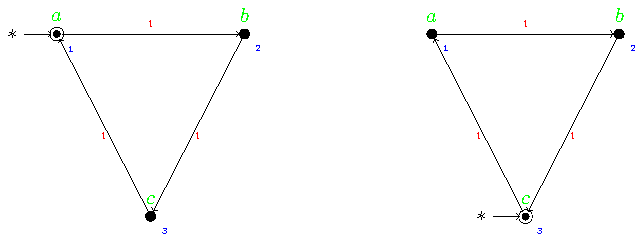
\includegraphics[scale=.8]{images/counterexample.pdf}
	\caption{Two TGs, $Q$ (left) and $R$ (right), having a different set of traces but the same embedding representation.}\label{fig:counterexample}
\end{figure}
\begin{example}
	If we use $\epsilon$ and $\nu$ as defined in Equations \ref{eq:epsilon}-\ref{eq:nu}, we might have a false positive for ``weak equality'' if $Q=(s,s,L,R,w)$ and $R=(s',s',L,R,w)$ are both cycle graphs with $s\neq s'$, $\textit{label}(s)\neq\textit{label}(s')$, $\textit{label}(s)\neq\varepsilon$, and $\textit{label}(s')\neq\varepsilon$. An intuitive example of such situation is presented in Figure \ref{fig:counterexample}: both graphs will have the same frequency for both subtraces and nodes, and therefore have the same  $\epsilon$ and $\nu$ by construction. By having different initial and accepting node with  different labels, we have $\mathcal{W}_0^{\aleph_0}(Q)=\Set{\textup{a(bca)}^n|n\in\mathbb{N}}$ and $\mathcal{W}_0^{\aleph_0}(R)=\Set{\textup{c(abc)}^n|n\in\mathbb{N}}$, thus implying $\mathcal{W}_0^{\aleph_0}(Q)\neq\mathcal{W}_0^{\aleph_0}(R)$ but $k_{\phi_{\mathcal{P}}}(Q,R)=1$ for $t_f=1$.
\end{example}


\begin{lemma}[Weak Equality]
	Given two TGs $P=(s,t,L,R,w)$ and $P'=(s',t',L',R',w')$ providing the same set of weighted traces, then $k_{\phi_{\mathcal{P}}}(P,P')=ww'$ for $t_f=1$.
\end{lemma}
\begin{proof}
	\xout{Given Proposition \ref{lem:rewritinglemma} and the positive definition of $\epsilon$ and $\nu$,  we have that $\norm{\hat{\epsilon}-\hat{\epsilon}'}{2}\to 0$ as well as $\norm{\hat{\nu}-\hat{\nu}'}{2}\to 0$, for which we can immediately close the goal.}
\end{proof}

\xout{As per previous observations, we know that} Two TGs should have the maximum dissimilarity when all the non $\varepsilon$-nodes have different labels, thus making it impossible to find an alignment, thus implying that they share an utterly dissimilar set of weighted traces:

\begin{lemma}[Strong Dissimilarity]
	Given two TGs $P=(s,t,L,R,w)$ and $P'=(s',t',L',R',w')$, $k_{\phi_{\mathcal{P}}}(P,P')=0$ iff. $P$ and $P'$ have a different set of labels with $t_f,w,w'>0$.
\end{lemma}
\begin{proof}
	\xout{If we exclude the trivial conditions $t_f=0$, $w=0$ or $w'=0$, the only condition when the kernel returns zero is when  $\Braket{\hat{\epsilon},\hat{\epsilon}'}=0$ and $\Braket{\hat{\nu},\hat{\nu}'}=0$. This implies that, when a component of $\epsilon$ (or $\nu$) is non-zero, the same component of $\epsilon'$ (or $\nu'$) is zero and viceversa. This directly requires that there is a different set of labels associated to the nodes. }
\end{proof}

As a corollary of the two lemmas, we have that the proposed embedding performs weakly-ideally, as the equality condition holds only on a relaxed form.

Last, under the assumption that a TG is approximately characterized by $\epsilon$ and $\nu$, we might expect that the TG similarity is characterized by the sum of the distance of both embeddings. Therefore, we show that an increase in both distance embeddings approximately corresponds to a decrease in the kernel output and vice-versa.\yellownote{TODO (if required), establish the further approximation from such distributions and the actual expected ranking.}

\begin{lemma}\label{lem:approxRank}
	Given two TGs $P=(s,t,L,R,w)$ and $P'=(s',t',L',R',w')$ having respectively the embeddings $(\epsilon,\nu)$ and $(\epsilon',\nu')$, we have that the kernel $k_{\phi_{\mathcal{T}}}$ induces an inverse ranking of $\norm{\hat{\epsilon}-\hat{\epsilon}'}{2}+\norm{\hat{\nu}-\hat{\nu}'}{2}$:
	$$k_{\phi_{\mathcal{T}}}(P,P')\appropto 2-(\norm{\hat{\epsilon}-\hat{\epsilon}'}{2}+\norm{\hat{\nu}-\hat{\nu}'}{2})$$
\end{lemma}
\begin{proof}
	\xout{Let us use $T=t_f^{|R>0|+|R'>0|}$, $\omega=ww'$, $V=\norm{\hat{\nu}-\hat{\nu}'}{2}$, and $E=\norm{\hat{\epsilon}-\hat{\epsilon}'}{2}$ as shorthands. The goal can be rewritten as $k_{\phi_{\mathcal{T}}}(P,P')\appropto 2-(E+V)$. Given that the embeddings $(\epsilon,\nu)$ and $(\epsilon',\nu')$ are normalized kernel function $k_{\phi_{\mathcal{P}}}$ and that they are always positive definite, then we have that $0\leq E +V\leq 2$, so $0\leq 2-(E+V)\leq 2$. Using Proposition \ref{lem:rewritinglemma}, we can write $k_{\phi_{\mathcal{P}}}(P,P')$ as follows:}
	$$\Rcancel{\left(1-\frac{E}{2}\right)\omega T+\left(1-\frac{V}{2}\right)T=T\left(\omega+1-\frac{E\omega+V}{2}\right)}$$
	\xout{Given that the embeddings $(\epsilon,\nu)$ and $(\epsilon',\nu')$ are normalized in $k$ and that they are always positive definite,  we also have that $0\leq E\omega +V\leq 2$ where $0\leq \omega\leq 1$. We can also write  $0\leq \omega+1-\frac{E\omega+V}{2}\leq \frac{2}{T}$. For $\omega,T=1$, we have that $k_{\phi_{\mathcal{P}}}(P,P')=2-\frac{(E+V)}{2}$. Thus, $0<\omega,T<1$ approximates the expected ranking. }
\end{proof}

\ADD{Such lemma is going to be empirically evaluated in our experiment section.}
